\chapter{Implementace frontendu}
Frontend byl vyvíjen jako single-page application pomocí programovacího jazyku JavaScript a knihovny React.
A byl navržen tak, aby byl jednoduše ovladatelný, přehledný a především velmi rychlý.

\section{Hostující server}
Celá aplikace frontendu je uložena na serveru, včetně zdrojových kódů.
Uživatel si ale stahuje pouze zkompilovanou aplikaci a případné externí zdroje.
\subsection{Kompilace}
Ačkoliv je JavaScript skriptovací jazyk a kompilaci provádí až za běhu, tak je možné
jej zkompilovat předem. Při této kompilaci knihovny \textbf{webpack} a
\textbf{babel} provedou několik zásadních kroků. Nejdůležitější z nich jsou
převedení kódu na ECMAScript 5 (kvůli zpětné kompatibilitě), přetřídění a sloučení
knihoven do jednoho zdrojového souboru (JavaScript se k uživateli dostane při prvním dotazu na server) a
minifikace výsledného souboru, jež dokáže inteligentně projít kód a optimalizovat jeho textovou délku,
čímž výrazně sníží čas potřebný k načtení stránky.

\subsection{NPM}
Celá aplikace má strukturu balíčku NPM (node package manager), tudíž ji lze snadno
spustit kdekoliv, kde je nainstalovaný \textit{nodejs} (ve verzi minimálně 16.0).
Zároveň udržuje pomocí souboru \textbf{package.json} přehled o potřebných knihovnách (dependencies) a
obsahuje též různé spouštěcí scripty, např. script pro build produkční verze aplikace.

\section{Knihovny}
Aplikace se skládá z více než tisíce knihoven a modulů, tudíž se podíváme
pouze na ty největší a nejdůležitější z nich.

\subsection{React}
Tato JavaScriptová knihovna byla vyvinuta společností Facebook a slouží pro tvorbu uživatelského rozhraní.\\
Jejím základem je vykreslování pomocí technologie \textit{single-page application} a je vhodná zejména pro aplikace, kde se často mění data.
Využívá pozměněné JavaScriptové syntaxe známe jako JSX (JavaScript XML), která umožňuje
pracovat s HTML tagy uvnitř JavaScriptového kódu, bez nutnosti práce s DOM objektem.\\
Výhodou single-page aplikace je pak i optimalizovaná práce s DOM objektem, který je bottleneckem
(úzkým hrdlem) při nesprávném použití (nebo lépe řečeno, při valné většině použití, které
něco s DOM objektem dělá).

\subsection{Material-UI}
Společnost Google (aktuálně Alphabet Inc.) se v roce 2014 rozhodla sjednotit svou grafickou podobu a
vyvinula designový jazyk, jež se stal příručkou jak vytvářet uživatelsky přívětivé aplikace
(nejen na webu, ale třeba i v aplikaci na mobilním telefonu nebo tabletu).
Základem tohoto stylu je realistická práce se světlem a uživatelskou interakcí.
Design je to odlehčený a intuitivní. Součástí tohoto grafického jazyka jsou i
lehce čitelné fonty (například Roboto), pochopitelné ikonky a systém barev a jejich kombinací.

\subsection{i18n (internacionalizační knihovna)}
Jelikož je projekt mířen i na nečeské uživatele, vyskytla se potřeba rozhraní překládat.
Jednoduchým přístupem by bylo zkompilovat několik aplikací, každou pro jiný jazyk, tudíž
by se překlad odehrával na straně serveru. Bohužel to není optimální řešení, a
tudíž byla využita knihovna \textit{i18n}, jež funguje na podobném principu jako single-page application a
to sice, že dokáže měnit překlad stránky bez nutnosti stránku přenačíst, a zároveň hlavní aplikace
neobsahuje všechny jazyky při prvním načtení. Jazyky se postupně dostahují dle preference uživatele
(vše samozřejmě na pozadí bez uživatelského zásahu).\\
Velkou výhodou tohoto systému může být například situace, kdy je potřeba přeložit kus textu na stránce,
případně sehnat anglický ekvivalent a nechceme přenačtením stránky přijít o již vyplněná data.

\subsection{Babel}
Jak už bylo zmíněno výše, aplikace se kompiluje a za tuto část je zodpovědná právě knihovna Babel.\\
Hlavní výhodou je kompilace kódu ve verzi ES6+ (EcmaScipt v6, neboli JavaScript v6) do verze
ES5 (EcmaScipt v5, neboli JavaScript v5).
Tímto převodem získáme zpětnou kompatibilitu pro starší JavaScriptové enginy.

\subsection{Webpack}
Aby se z tak obrovského množství knihoven a souborů stal jediný spustitelný soubor, pomůže nám
knihovna Webpack, která dokáže kód zkomprimovat a sjednotit. Touto optimalizací si ušetříme
množství dotazů, jež bude muset náš server přijmout (a ekvivalentně s tím uživatel odeslat).\\
Zároveň nám umožňuje používat formát \textbf{SCSS}, což je nadstavba nad klasickým CSS, jež 
rozpoznávají prohlížeče, a dovoluje nám takto vytvářet \textbf{stylovací moduly}.

\section{Rozhraní}
Jelikož se jedná o složitější systém a všechno nemůže být \uv{naházené} v jediném souboru, 
je použita hierarchie o třech hlavních úrovních. Nejvýše je \textbf{hlavní soubor celého webu}, který
provádí routing (směrování) a obaluje celou aplikaci pomocnými wrapery (např. \textit{i18n}
překladač, \textit{Mui} pro jednotný styl, \textit{SnackbarProvider} pro vyskakovací
toasty a \textit{CookiesProvider} pro jednotný přístup ke cookies). Pod ním jsou jednotlivé
\textbf{scény} neboli stránky diametrálně rozdílných vlastností a funkcionalit používající poslední
úroveň, jež jsou \textbf{komponenty}, malé na sobě nezávislé černé krabičky\footnote{černa krabička -
metoda u které není znám přesný algoritmus pro převod vstupních dat na výstupní}
poskytující určitou funkcionalitu.


\subsection{Scény}
Většina scén má klasické pojmenování, ale najdeme zde i uživatelsky atraktivní přesná
pojmenování scén podle účelu jako je \uv{Vyhledávátko}, \uv{Zobrazovátko} nebo \uv{Upravovátko}.

\subsubsection{Admin}
Administrační rozhraní je přístupné pouze s oprávněním \uv{execute}.
Zde může administrátor nebo správce uživatelů vytvářet nové účty nebo
konfigurovat stávající.\\
Protože se hesla v databázi ukládají zahešovaná, tak je nelze zobrazit ani administrátorovi.
Dala by se přidat funkcionalita pro jejich crackovaní, aby se nalezli uživatelé se
slabými hesly, ale to by bylo zbytečné plýtvání serverovými prostředky.
\begin{figure}[H]
	\centering
	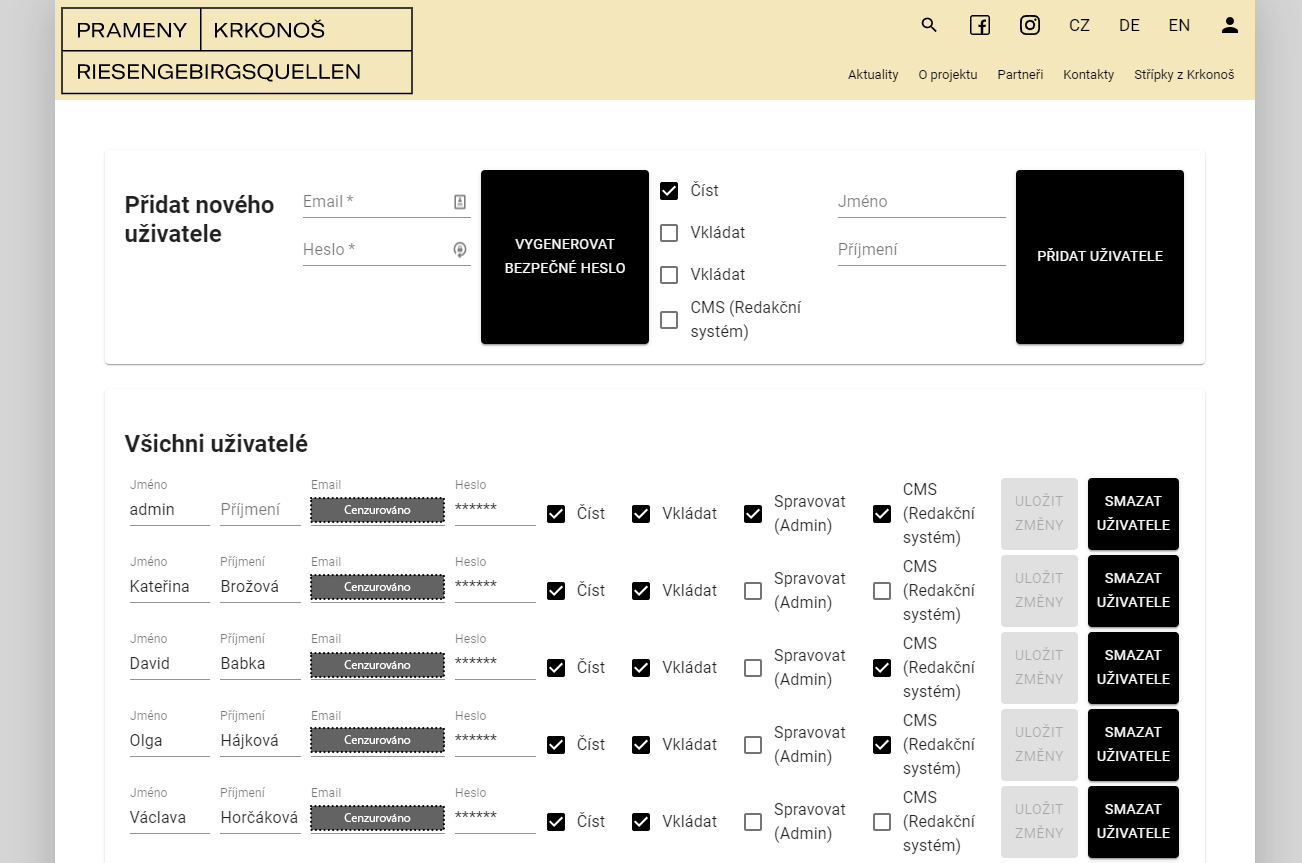
\includegraphics[width=.8\linewidth]{img/adminScene.png}
	\caption{Frontend administrační scény}
\end{figure}

\subsubsection{CMS}
Vytváření a editace obsahu stránek se provádí v redakčním systému (Content Management System, zkráceně CMS).
Do něj se uživatel dostane pouze po přihlášení a s platnými právy pro redakční systém.\\
Úpravy redaktor provádí v prostředí WYSIWYG (a anglického \uv{What you see is what you get}, přeloženo \uv{Co vidíš, to dostaneš}).
V pravém panelu pak zadá název, případně krátký popis, který se hodí např. pro aktuality a kategorii.\\
WYSIWYG editor podporuje velkou škálu stylování a formátování. Velkou výhodou je možnost nahrávání obrázků,
kdy se po přetažení automaticky uloží na server do složky \textit{uploads} a jejich odkaz se vloží do stránky.
\begin{figure}[H]
	\centering
	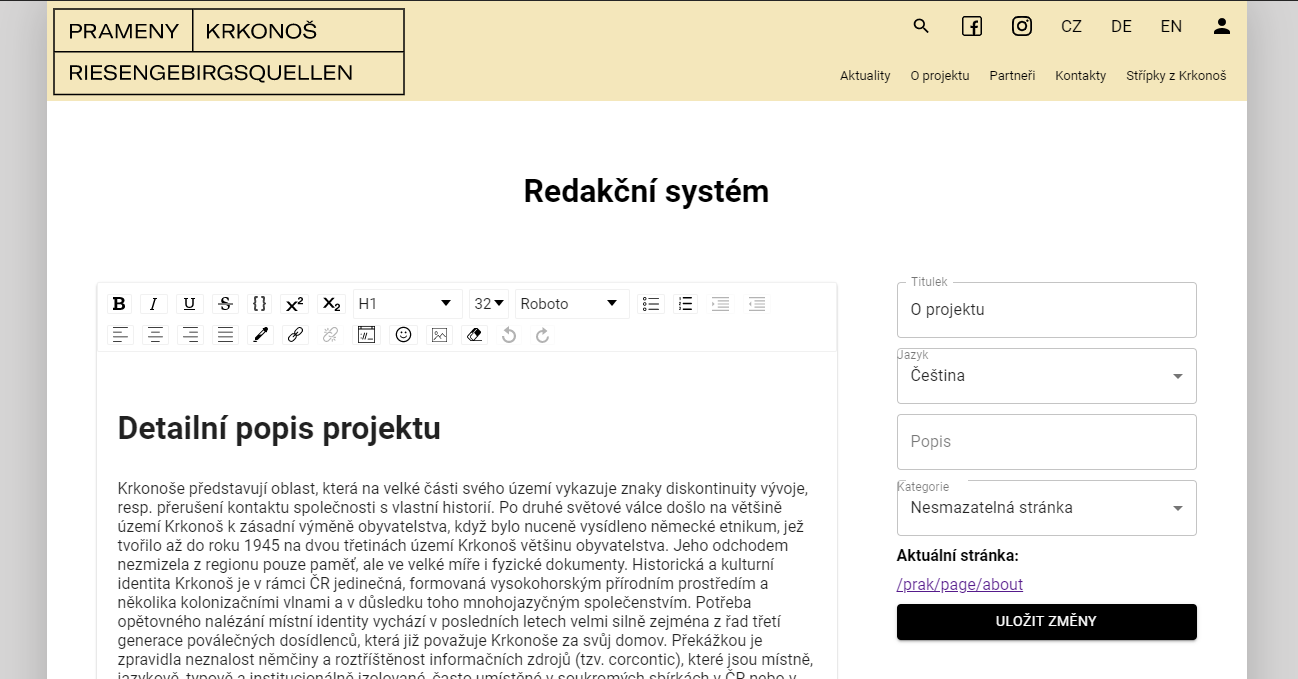
\includegraphics[width=.8\linewidth]{img/cmsScene.png}
	\caption{Frontend scény pro editaci stránek (CMS)}
\end{figure}

\subsubsection{Domovská stránka}
Výchozí stránka, na kterou se uživatel dostane, pokud nezadá přesnější cestu v url, je domovská stránka.\\
Na této stránce uživatel najde dynamické zobrazování novinek a krátkého popisu v hormím panelu a stránku
s názvem \uv{homepage}, což je obyčejná stránka editovatelná v redakčním systému, a dovoluje tedy
redaktorům měnit i domovskou stránku.
\begin{figure}[H]
	\centering
	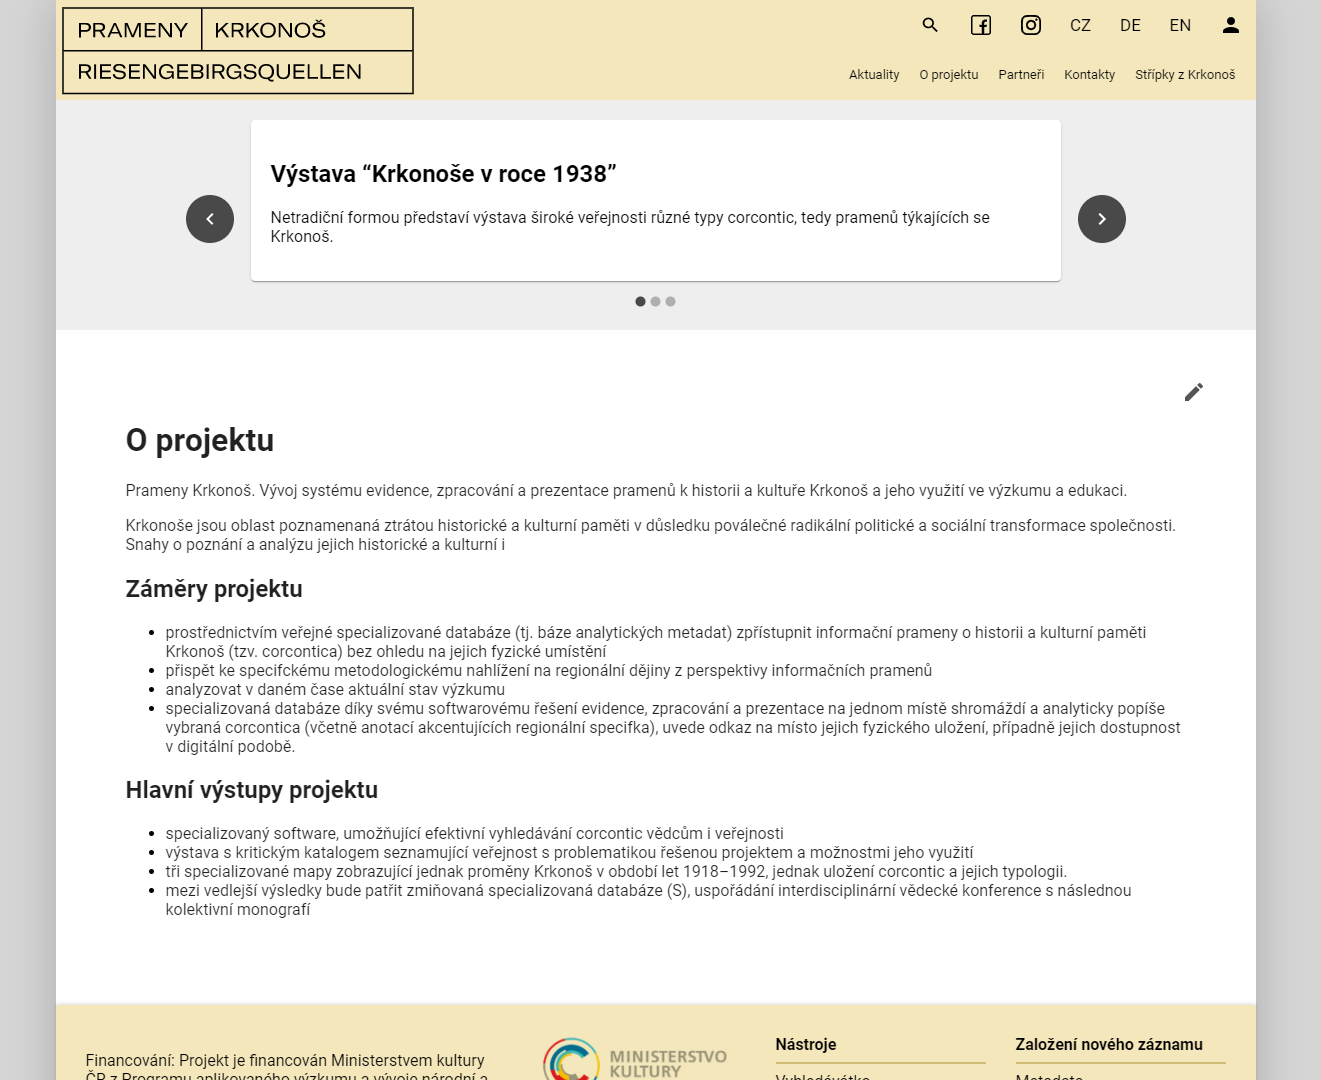
\includegraphics[width=.8\linewidth]{img/homeScene.png}
	\caption{Frontend hlavní stránky aplikace}
\end{figure}

\subsubsection{Zobrazení stránky}
Každá stránka vytvořená v redakčním systému je přístupná na url adrese \texttt{.../prak/page/\#jmenoStranky}.
Zde si ji mohou uživatelé zobrazit. Pokud má uživatel i právo pro redakční systém,
tak se mu v pravém horním rohu zobrazí ikonka pro editaci, díky které se snadno dostane do
redakčního systému pro danou stránku.
\begin{figure}[H]
	\centering
	
\includegraphics[width=.8\linewidth]{img/pageScene.png}
	\caption{Zobrazení normální informativní stránky}
\end{figure}

\subsubsection{Kontaktní formulář}
Pro zpětnou vazbu či otázky k projektu, mohou návštěvníci využít kontaktní formulář.
\begin{figure}[H]
	\centering
	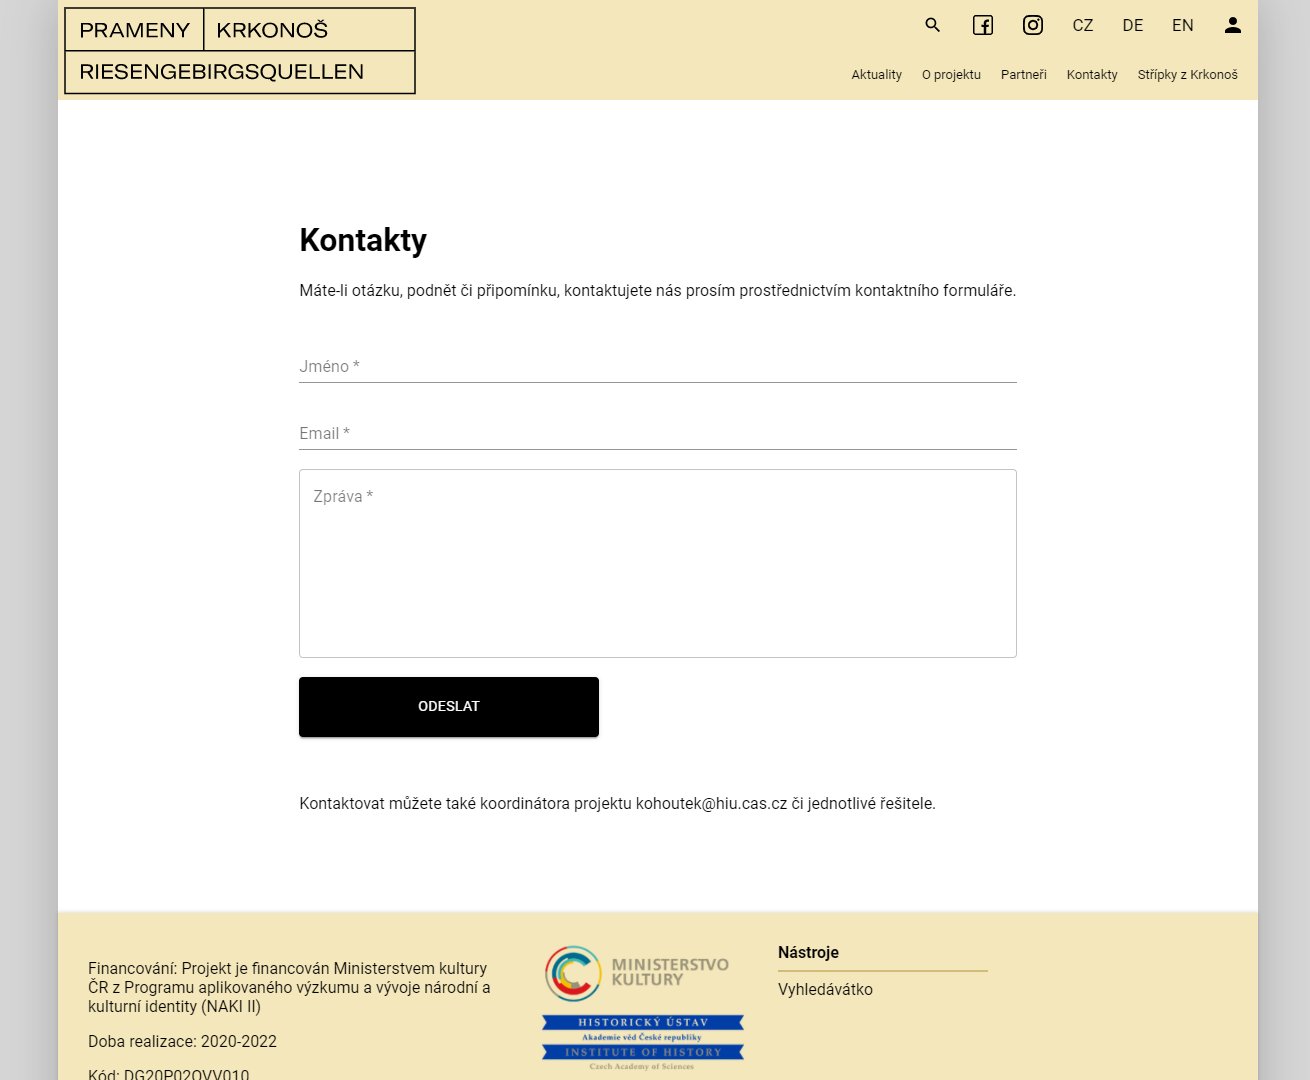
\includegraphics[width=.8\linewidth]{img/contactScene.png}
	\caption{Kontaktní formulář}
\end{figure}

\pagebreak
\subsubsection{Vyhledávátko}
Pomocí ikonky lupy v hlavičce se dostaneme do vyhledávacího prostředí.\\
Po výběru, kde chceme hledat, se nám načtou políčka k vyplnění. Uživatel do nich může zadat
libovolný výraz, a to s podporou regexp syntaxe. Ihned při vyplňování se načítá až pět
prozatím nejvhodnějších výskytů hledání. Při kliknutí na tlačítko \uv{vyhledat} se provede
vyhledání všech odpovídajících záznamů.\\
Nalezené záznamy se objevují v tabulce pod vyhledávacím polem.
Tabulka dokáže záznamy třídit po kliknutí na hlavičku příslušného sloupce.
Po kliknutí na záznam se otevře editační prostředí pro vybraný záznam.
\begin{figure}[H]
	\centering
	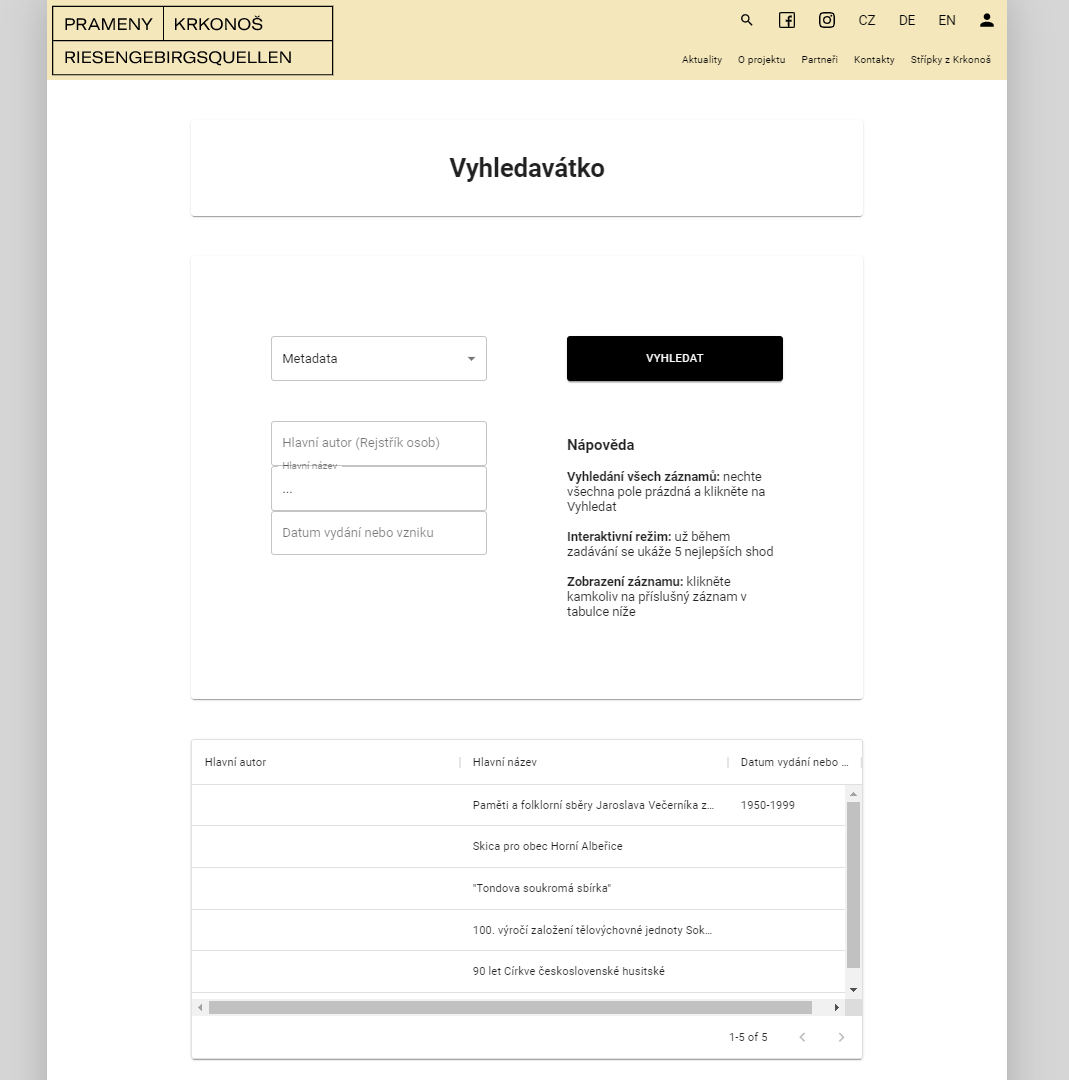
\includegraphics[width=.8\linewidth]{img/searchScene.png}
	\caption{Frontend Vyhledávátka}
\end{figure}

\pagebreak
\subsubsection{Zobrazovátko}
Záznam uložený v databázi si je možné zobrazit přes toto rozhraní, poté co
se k němu dostaneme přes vyhledávací rozhraní nebo pomocí unikátního
url linku, který se po vytvoření záznamu již nezmění.
\\
Po načtení se uživateli zobrazí záznam tak, jak je uložen v databázi, případně
s přeloženými názvy, pokud to je pomocí spodního přepínače povolené.
Dole jsou též dvě tlačítka pro smazání záznamu a editaci záznamu, jež uživatele
přesune do editačního rozhraní s aktuálním záznamem (samozřejmě jen pokud 
má dostatečná oprávnění).
\begin{figure}[H]
	\centering
	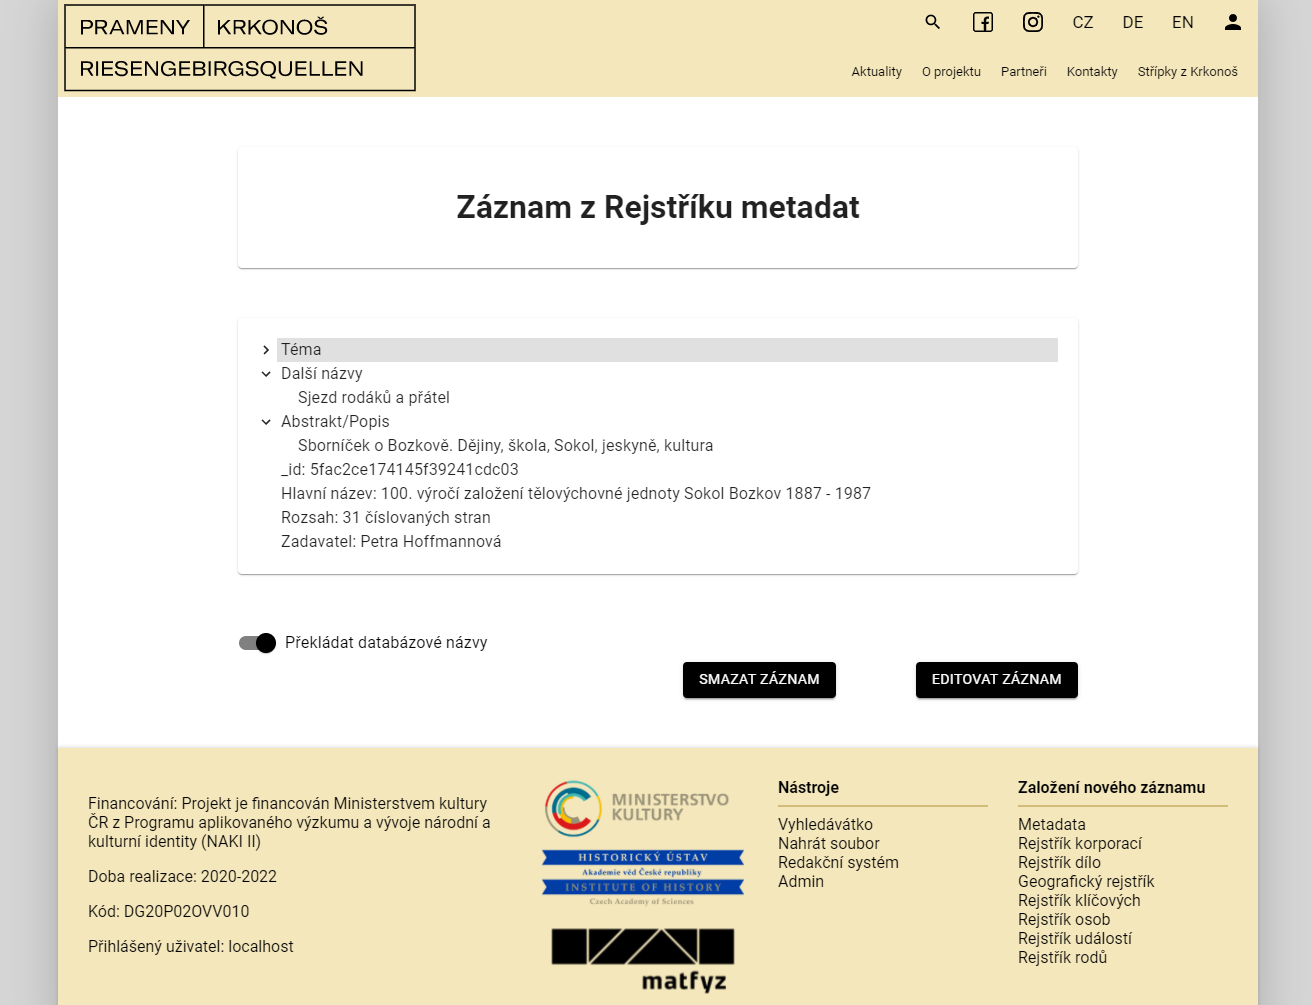
\includegraphics[width=.7\linewidth]{img/showScene.png}
	\caption{Frontend Zobrazovátka}
\end{figure}


\subsubsection{Přihlašování}
Pokud uživatel klikne na ikonku postavičky vpravo v hlavičce, nebo se pokusí dostat
na stránku, ke které nemá oprávnění, je přesměrován do přihlašovacího prostředí.
Pokud se na této stránce přihlásí, nebo již přihlášen byl, zobrazí se mu podrobnosti o jeho účtu,
včetně dostupných oprávnění.\\
\begin{figure}[H]
	\centering
	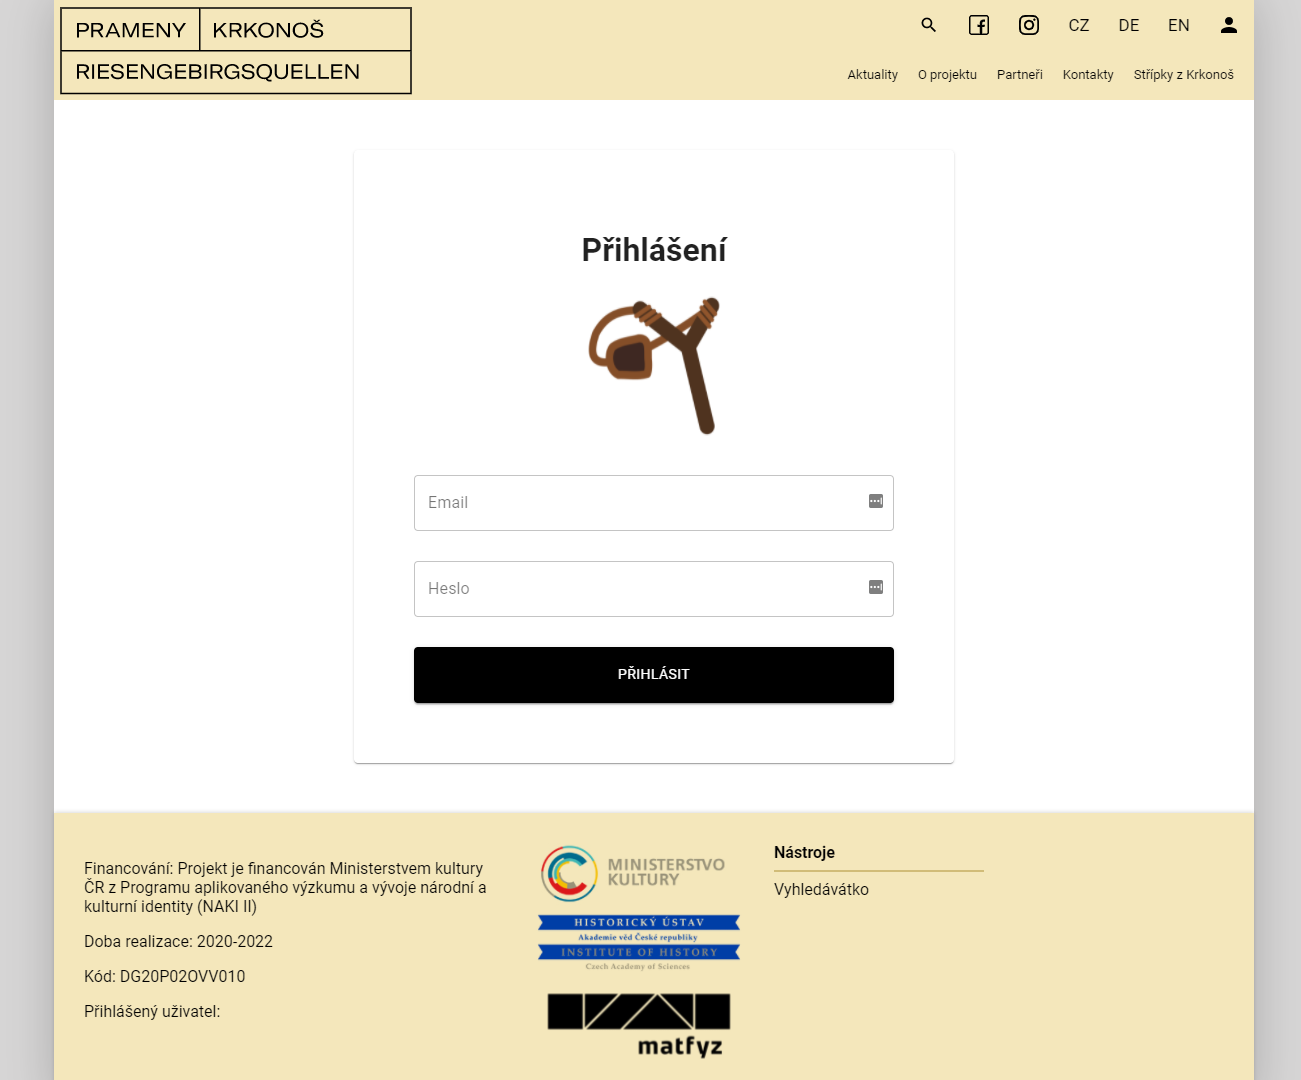
\includegraphics[width=.49\linewidth]{img/loginSceneB.png}
	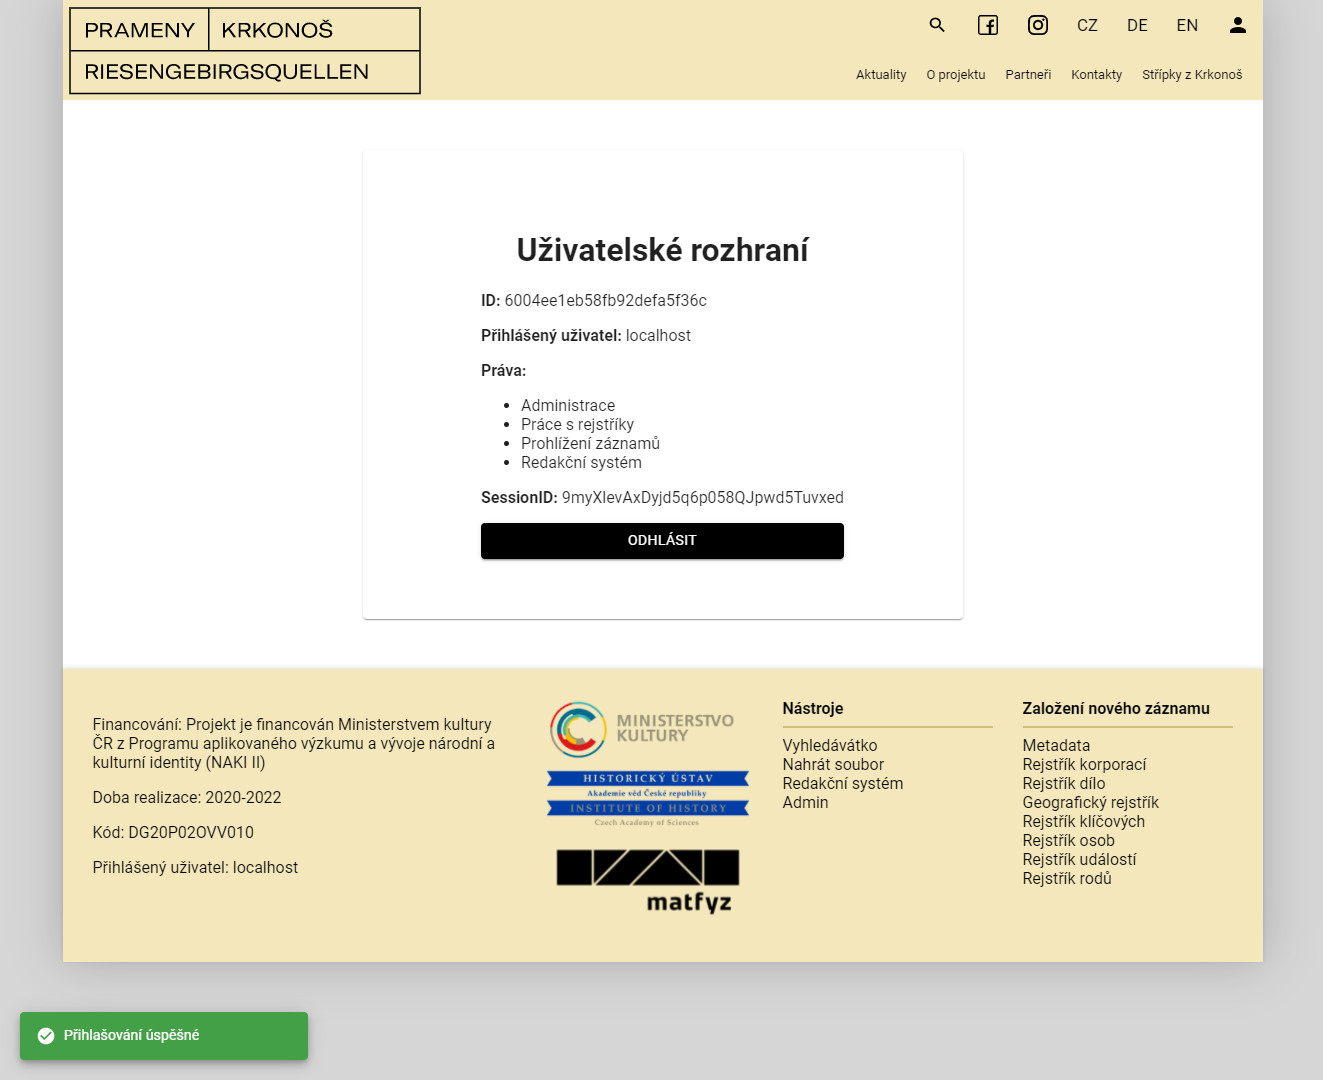
\includegraphics[width=.5\linewidth]{img/loginSceneA.png}
	\caption{Přihlašovací stránka vlevo a stránka s informacemi o přihlášeném uživateli vpravo}
\end{figure}


\subsubsection{Upravovátko}
V tomto prostředí je možné záznam upravovat a jedná se o nejkomplikovanější scénu tohoto projektu.\\
Každý typ záznamu a každý podtyp metadatové struktury má vlastní příslušná datová pole.
Ty, které umožňují mít více hodnot, mají vpravo od sebe tlačítka plus a mínus,
jehož vertikální velikost určuje velikost bloku, jež je jedním celkem. Plusové tlačítko přidává
další datové pole, zatímco mínus datové pole vyprázdní a poté odebere z náhledu.
\\
Datová pole jsou roztříděna do menších bloků a lze tlačítkem minimalizovat
(vyplněná data se nezahodí, ale pouze skryjí), aby uživateli usnadnily orientaci.
Po minimalizaci, resp. maximalizaci, bloku může dojít k převážení
sloupců a některé bloky tak mohou střídat levý a pravý sloupec, tak aby celková stránka byla co nejkratší
a prázdného místa bylo co nejméně.\\
Některé záznamy mají možnost nahrát přílohu, ta se aktivuje po kliknutí na tlačítko uploadu, s ikonkou šipky
směrem nahoru. Nahraný soubor se ihned přenáší na server a do příslušného pole automaticky 
zaznamená aktuální url nahrávaného souboru.\\
Po kliknutí na tlačítko Nahrát se buď objeví červené vyskakovací okno s chybou, proč záznam nelze uložit
(většinou zapříčiněný zadáním unikátního názvu, jež již je v databázi uložen).
Nebo se stránka znovu přepne do \textit{Zobrazovátka} a vyskočí zelené potvrzovací okénko.
\begin{figure}[H]
	\centering
	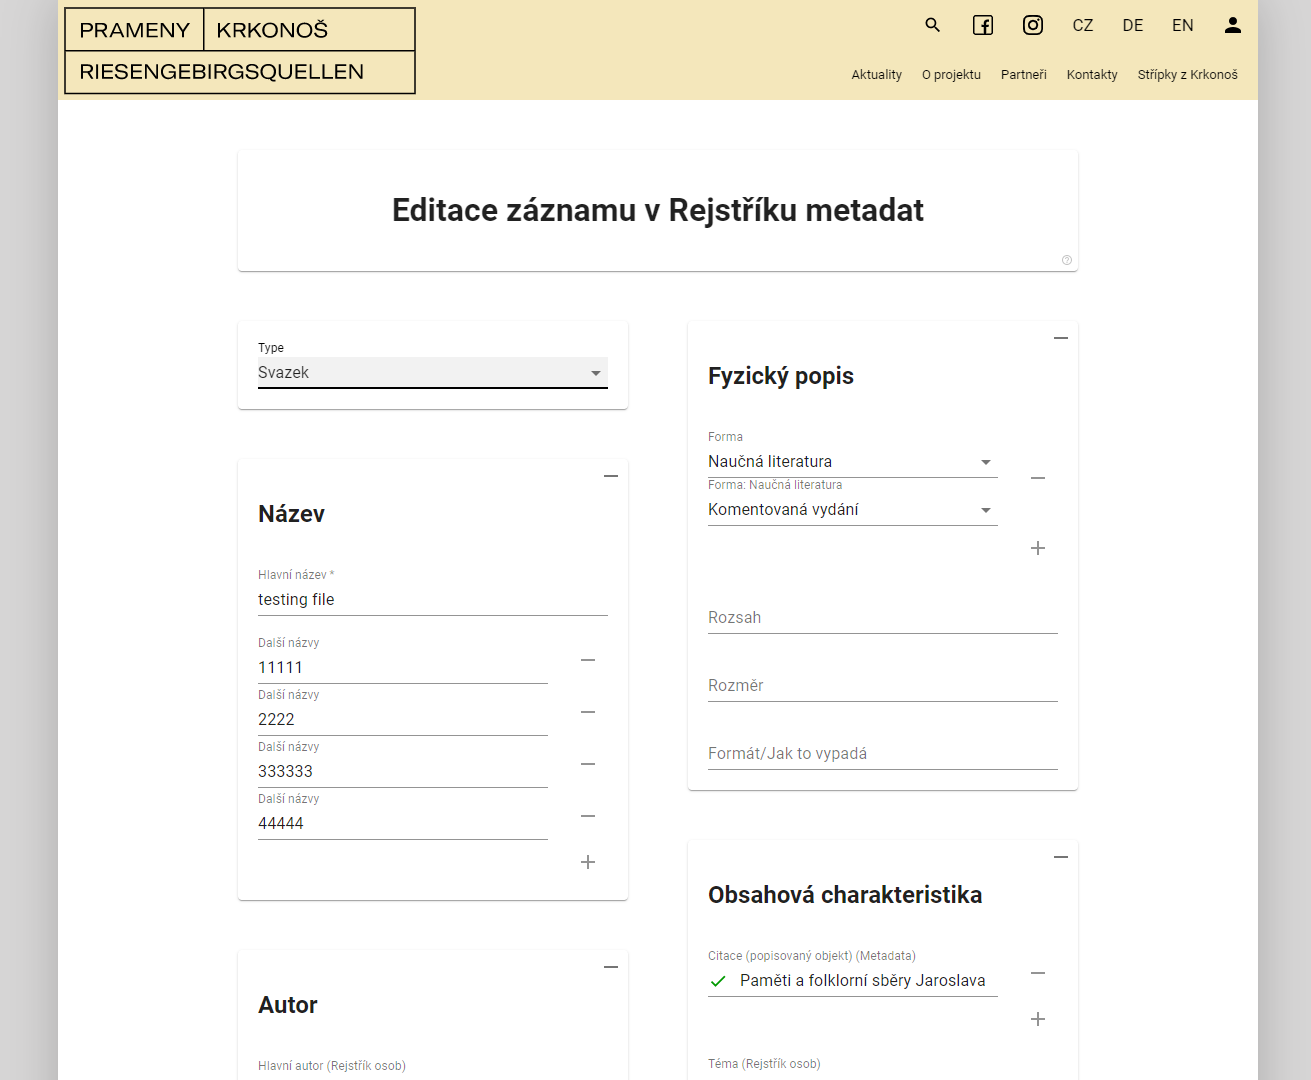
\includegraphics[width=.8\linewidth]{img/editScene.png}
	\caption{Frontend Upravovátka}
\end{figure}

\pagebreak
\subsection{Komponenty}
Komponenty jsou vlastně zapouzdřené třídy, které se dají použít vícekrát.
Každá komponenta je vhodná pro React systém a většinou je psaná bez tzv. hooků
(alternativní přístup k proměnným u komponent typu funkce, namísto typu třída).

\subsubsection{ComboBox}
\begin{wrapfigure}{r}{0.4\linewidth}
	\centering
	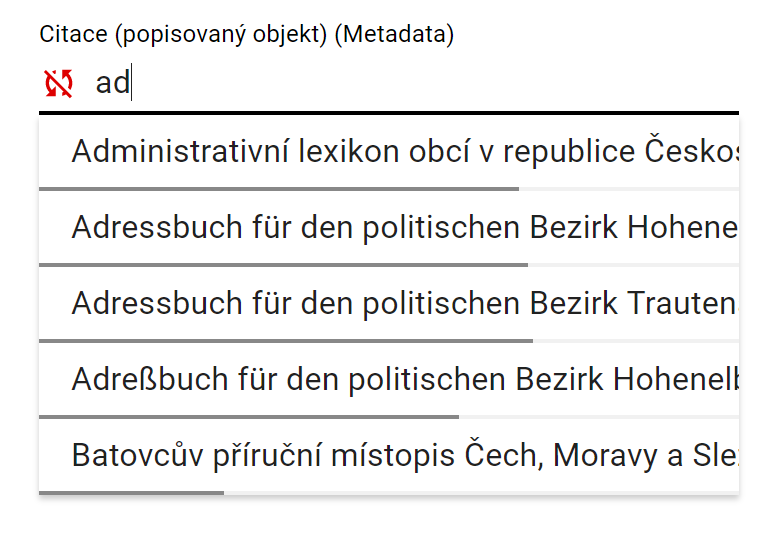
\includegraphics[width=\linewidth]{img/ComboBox.png}
	\caption{Komponenta ComboBox}
\end{wrapfigure}
ComboBox je textové pole, které při vyplňování realtime vyhledává v databázi vyhovující shody,
které zobrazuje ve formě nabídky pod tímto textovým vstupem. Po kliknutí na nabízenou položku se
do pole vyplní hodnota a na pozadí se do pole uloží ID záznamu (to se poté odesílá na server).
Dokud uživatel některý ze záznamů nevybere, pole není v konzistentním stavu a nemá možnost se
odeslat na server, což značí ikonka

\includegraphics[height=\fontcharht\font`\B]{img/notSynced.png}.
V případě, že pole má přiřazené ID záznamu a zobrazuje název, rozsvítí se ikonka

\includegraphics[height=\fontcharht\font`\B]{img/synced.png},
která značí že data z tohoto pole se při uložení správně odešlou na server.
Popisky často bývají dlouhé, a proto je zde i miniaturní posuvník, se kterým se
dá pohodlně pracovat pomocí najetí myši na políčko, přidržení klávesy \textit{Shift} a
točením kolečka na myši.

\subsubsection{Zápatí}
Jako každá správná stránka i tato má zápatí, jež obsahuje povinné údaje o projektu a
rychlé odkazy.\\
Jelikož se jedná o projekt MK ČR - NAKI, nalezneme zde povinné údaje, kód projektu a
loga sponzora, zadavatelů a vývojářů.
Níže je ukazatel aktuálně přihlášeného uživatele.
V pravé části jsou pak rychlé odkazy, které se zobrazují v závislosti na právech přihlášeného uživatele.
Nepřihlášený uživatel tudíž v této části uvidí pouze jedno menu \uv{Nástroje} s jedinou
položkou \uv{Vyhledávátko} a po přihlášení se (viz obrázek 5.11) menu rozroste o další rychlé odkazy.
\begin{figure}[H]
	\centering
	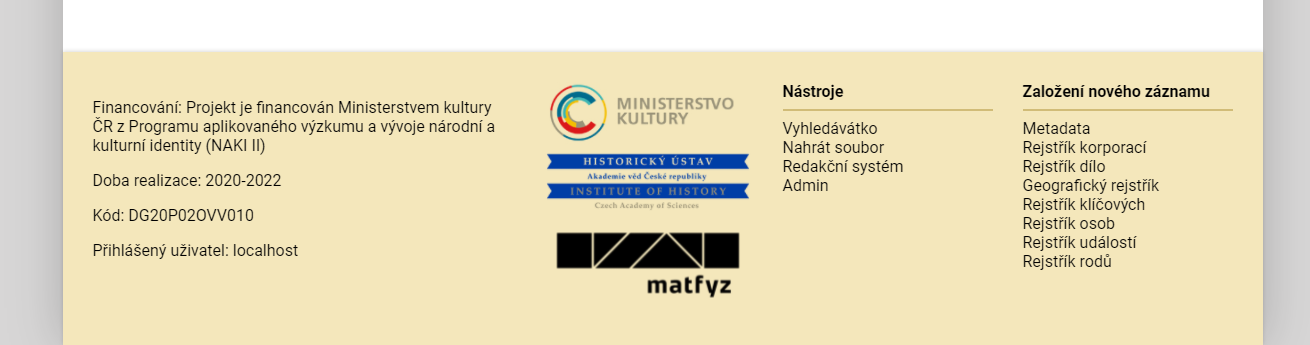
\includegraphics[width=.8\linewidth]{img/zapati.png}
	\caption{Zápatí stránky}
\end{figure}

\pagebreak
\subsubsection{Navigační menu}
V navigačním menu nalezneme rychlé odkazy na Vyhledávátko (tlačítko s ikonkou lupy),
Facebook a Instagram projektu Prameny Krkonoš a přihlašovací stránku. Tlačítka pro
přepínání mezi třemi jazyky. Níže pak důležité stránky projektu a některé kategorie
(např. kategorie Aktuality).
\begin{figure}[H]
	\centering
	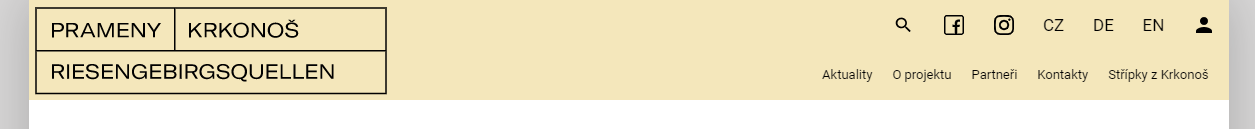
\includegraphics[width=.8\linewidth]{img/navigationBar.png}
	\caption{Navigační menu}
\end{figure}

\subsubsection{Textové pole s validací}
\begin{wrapfigure}{r}{0.4\linewidth}
	\centering
	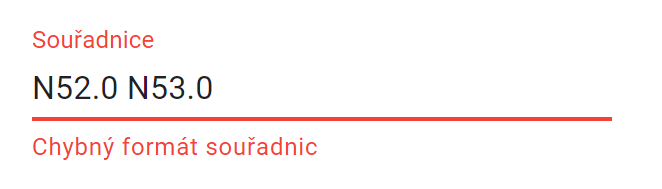
\includegraphics[width=\linewidth]{img/validationField.png}
	\caption{Pole s kontrolou validity dat}
\end{wrapfigure}
To, že uživatel zadává data ve srozumitelném formátu (tak aby je dokázal pochopit další
uživatel nebo aby je databáze správně interpretovala), je kontrolováno na straně klienta
(a po odeslání i na straně serveru).
V případě, že data požadovaný formát nemají, pod políčkem se zobrazí varovný nápis a
záznam nepůjde uložit, dokud všechna pole nejsou ve správném formátu.

\subsubsection{Pole pro nahrávání souborů}
\begin{wrapfigure}{r}{0.4\linewidth}
	\centering
	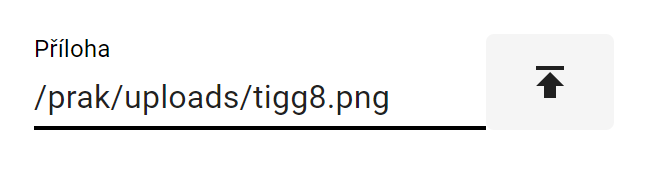
\includegraphics[width=\linewidth]{img/uploadField.png}
	\caption{Pole pro nahrávání souborů}
\end{wrapfigure}
U některých záznamů je užitečné uchovat přílohu ve formátu obrázku nebo dokumentu.\\
Tyto soubory lze nahrát na server a do databáze uložit pouze odkaz na jejich umístění,
protože databáze není stavěná na uchovávání obrázků a podobných relativně velkých souborů.

\subsubsection{Indexy}
Hlavní částí editačního rozhraní jsou indexové objekty, které určují, která pole
se mají zobrazit při různých typech záznamů. Pro každý typ je zde JSON soubor, ve kterém
je seznam polí a informace o nich. Mezi tyto informace patří především popisek, struktura, jak
data odeslat do databáze, nápověda přístupná pomocí malého otazníčku a nepovinná pole jako
požadavek na nenulovou hodnotu, nebo regexpový výraz pro kontrolu formátu dat.

\subsection{Moduly}
Funkcionalita, která není až tak často používána, se do hlavního souboru aplikace
nepřidává a tudíž čistý frontend žádné moduly nepodporuje. Moduly jsou výhradně načítány
ze serveru a neobsahují hlavní frontend.

\section{Lokalizace}
Překlad stránky do různých jazyků je řešen pomocí knihovny i18n, která je velmi efektivní a
zároveň poskytuje snadný způsob, jak texty překladu přidávat a editovat. 
Překlady navíc jsou rozloženy do více souborů a úrovní, takže se překlad velmi dobře
škáluje i na větší projekty.\\
Výsledkem jsou lokalizační soubory ve formátu JSON, které frontend aplikuje na požadovaných
místech. Pokud ovšem překlad chybí, použije se nejbližší možná interpretace, podobný jazyk nebo
zdrojová adresa překladu a vývojáři ukáže zprávu o chybějícím překladu.
\begin{figure}[H]
	\centering
	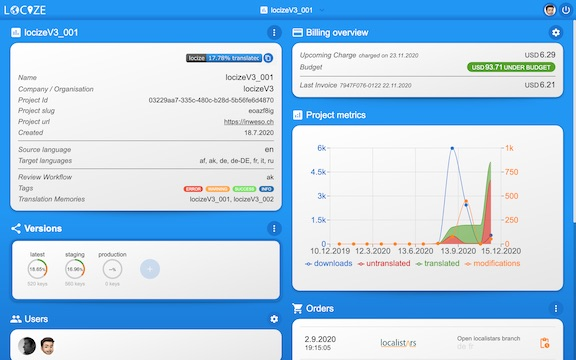
\includegraphics[width=.7\linewidth]{img/locize.jpg}
	\caption[Aplikace Locize umožňující správu překladů knihovny i18n, zdroj: \url{https://locize.com/}]{Aplikace Locize umožňující správu překladů knihovny i18n}
\end{figure}